\clearpage
\section{Note H}

\subsection{Prelude}

\subsubsection{Recall}

We have already seen how non-convex loss functions can arise
in regularized loss minimization problems.
\eg, linear regression with corrupted observations.

\subsubsection{Motivation}

There has been much interest in the study of non-convex regularizers too.
In the context of sparse linear regression,
the motivation for studying non-convex regularizers is quite natural,
as $l_1$-``norm'' is just a convex approximation of the $l_0$-``norm'',
but not necessarily a good approximation; see Figure~\ref{fig:norms}.

\begin{figure}[ht]
\centering
    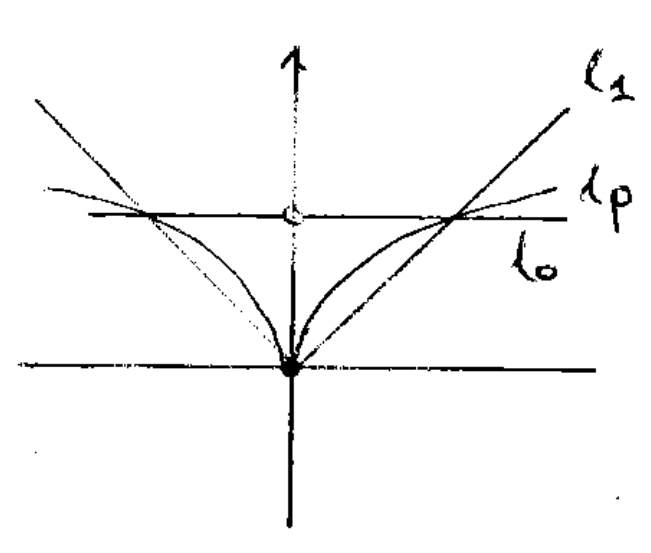
\includegraphics[width=0.32\linewidth]{fig/norms}
    \caption{\small Norms.}
    \label{fig:norms}
\end{figure}

A natural family of functions that interpolate between $l_0$ and $l_1$ is
the $l_p$-quasi-norm,
which is
\begin{equation}
    \|\theta\|_p^p=\sum_{i=1}^d|\theta_i|^p,\quad p\in(0,1).
\end{equation}
This is also known as the bridge penalty in the literature.
It can be verified that
\begin{equation}
    \lim_{\theta\to 0}(|\theta^p|)'=+\infty.
\end{equation}
such a feature is undesirable,
as it implies that $\hat\theta=0$ is always a local minimum to the problem
\begin{equation}
    \min_{\theta\in\real^d}\cL(\theta)+\lambda\|\theta\|_p^p.
\end{equation}
In particular,
there is no hope in bounding the statistical error $\|\hat\theta-\theta^*\|_2$
in general.

\subsection{Theme}

\subsubsection{An Assumption}

To circumvent this difficulty,
we consider regularizers $R_\lambda$ that are separable,
\ie,
\begin{equation}
    R_\lambda(\theta)=\sum_{i=1}^d R_\lambda(\theta_i),
\end{equation}
and satisfy the following properties.
\begin{ass}
Function $R_\lambda:\real\to\real$ satisfies the following:
\begin{enumerate}
    \item $R_\lambda(0)=0$ and $R_\lambda(t)=R_\lambda(-t)$ for all $t\in\real$.
    \item $R_\lambda$ is non-decreasing on $\real_+$.
    \item For $t>0$,
        the function $t\mapsto \frac{R_\lambda(t)}{t}$ is non-increasing in $t$.
    \item $R_\lambda$ is differentiable for all $t\ne0$
        and subdifferentiable at $t=0$ with
        $\lim_{t\searrow0}R_\lambda'(t)=\lambda L$ for some $L>0$.
    \item There exists a $\mu>0$ \st
        $t\mapsto R_{\lambda,\mu}(t)=R_\lambda(t)+\frac{\mu}{2}t^2$ is convex.
\end{enumerate}
\end{ass}

Both (1) and (2) are rather standard.
If $R_\lambda$ is concave on $\real_+$ and satisfies (1),
then it satisfies (3).
Condition (4) rules out those regularizers that have unbounded derivatives
at zero or are not differentiable at some $t\ne0$.
Lastly,
condition (5) sayas that $R_\lambda$ cannot be ``too non-convex''.

An interesting consequence of the above assumption is that
the function $R_\lambda$ is implementing a thresholding rule.
To see this,
define
\begin{equation}
    \lambda^*=\inf_{t>0}\bigg\{\frac{t}{2}+\frac{R_\lambda(t)}{t}\bigg\}.
\end{equation}
Observe that,
\begin{equation}
    0=\argmin_t\bigg\{\frac{(z-t)^2}{2}+R_\lambda(t)\bigg\}\quad
    \text{iff}\quad|z|\le\lambda^*.
\end{equation}
This follows from the fact that
\begin{equation}
    \frac{(z-t)^2}{2}+R_\lambda(t)-\frac{z^2}{2}
        =t\bigg(\frac{t}{2}+\frac{R_\lambda(t)}{t}-z\bigg).
\end{equation}

As a first example,
it can be readily verified that $R_\lambda(t)=\lambda|t|$
satisfies the above properties.
As it turns out,
so does many other widely used regularizers.

\begin{ex}[Smoothly Clipped Absolute Deviation (SCAD)]
\todo
\end{ex}

\begin{ex}[Minimax Concave Penalty (MCP)]
\todo
\end{ex}

\subsubsection{Consequences of Assumption}

Let us now collect some useful consequences of the properties in the assumption.
\begin{pro}
Under the assumption,
$R_\lambda$ is $\lambda L$-Lipschitz.
Moreover,
\begin{equation}
    \lambda L\|\theta\|_1\le R_\lambda(\theta)+\frac{\mu}{2}\|\theta\|_2^2\quad
    \forall\theta\in\real^d.
\end{equation}
\end{pro}
\begin{proof}
\todo
\end{proof}

The next proposition shows how $R_\lambda$ interacts with the $l_1$-norm
on sparse vectors.
\begin{pro}
Under the assumption,
let $\theta\in\real^d$ and $S$ be the index set of the $k$ largest elements
of $\theta$ in magnitude.
Then for any $\xi>0$,
we have
\begin{equation}
    \xi R_\lambda(\theta_S)-R_\lambda(\theta_{S^c})\le
        \lambda L\;\big(\xi\|\theta_S\|_1-\|\theta_{S^c}\|_1\big).
\end{equation}
Moreover,
if $\theta^*\in\real^d$ is $k$-sparse,
then for any $\theta\in\real^d$,
we have
\begin{equation}
    R_\lambda(\theta^*)-R_\lambda(\theta)\le
        \lambda L\;\big(\|\Delta_S\|_1-\|\Delta_{S^c}\|_1\big),
\end{equation}
where $\Delta=\theta-\theta^*$ and $S$ is the index set of the $k$
largest elements of $\Delta$ in magnitude.
\end{pro}
\begin{proof}
\todo
\end{proof}

\subsection{Finale}

Now let us consider the following regularized loss minimization problem.
\begin{equation}\label{eq:h1}
    \min_{\|\theta\|_1\le R}\big\{\cL(\theta)+R_\lambda(\theta)\big\},
\end{equation}
where $R_\lambda$ satisfies the assumption.
Since \eqref{eq:h1} is non-convex in general,
we are interested in bounding the statistical error $\|\tilde\theta-\theta^*\|_2$
for any $\tilde\theta\in\real^d$ satisfying the first-order optimality condition
of \eqref{eq:h1},
which is given by
\begin{equation}
    \big(\nabla\cL(\tilde\theta)+\nabla R_\lambda(\tilde\theta)\big)^T(\theta-\tilde\theta)
        \ge0\quad\forall\|\theta\|_1\le R.
\end{equation}
Toward that end,
we need a \emph{restricted strong convexity} (RSC)-type condition,
as our previous studies suggest.

\subsubsection{RSC Condition}

\begin{define}
We say that $\cL$ satisfies the RSC condition with parameters
$\alpha_1,\alpha_2>0,\tau_1,\tau_2\ge0$, if
\begin{equation}
    \big(\nabla\cL(\theta^*+\Delta)-\nabla\cL(\theta^*)\big)^T\Delta\ge
    \begin{cases}
        \alpha_1\|\Delta\|_2^2-\tau_1\frac{\log d}{n}\|\Delta\|_1^2 &\text{if }~\|\Delta\|_2\le1,\\
        \alpha_2\|\Delta\|_2-\tau_2\sqrt{\frac{\log d}{n}}\|\Delta\|_1 &\text{if }~\|\Delta\|_2\ge1.\\
    \end{cases}
\end{equation}
\end{define}

The RSC condition above consists of two inequalities,
instead of just on in the RSC conditions we introduced before.
It actually subsumes the previously introduced RSC conditions.
Furthermore,
it allows us to tackle more general (non-convex) loss functions.
For further discussions,
see~\cite{loh2015regularized}.

\subsubsection{Statistical Error Bound}

Using the above RSC condition,
we can establish the following result on the statistical error.
\begin{thm}
Suppose that $R_\lambda$ satisfies the assumption,
$\cL$ satisfies the RSC condition with $\alpha_1>\frac{\mu}{2}$,
and $\theta^*$ is feasible for \eqref{eq:h1}.
Provided
\begin{equation}
    \frac{4}{L}\max\bigg\{\|\nabla\cL(\theta^*)\|_\infty,
        \alpha_2\sqrt{\frac{\log d}{n}}\bigg\}\le\lambda\le\frac{\alpha_2}{{6LR}},
\end{equation}
and
\begin{equation}
    n\ge\frac{16R^2\max\{\tau_1^2,\tau_2^2\}}{\alpha_2^2}\log d,
\end{equation}
every $\tilde\theta$ satisfying the first order optimality condition of
\eqref{eq:h1} satisfies
\begin{equation}
    \|\tilde\theta-\theta^*\|_2\le\frac{3\lambda L\sqrt{k}}{2\alpha_1-\mu},
\end{equation}
where $k=\|\theta^*\|_0$.
\end{thm}
\begin{proof}
\todo
\end{proof}
